%!TEX root = Bericht.tex
\graphicspath{{graphics/HMI/}{graphics/control_modes/}}
\chapter{Finding a Hardware and Software Solution}
\label{cha:findHardSoftSolution}
In the following it is described how the previously defined control modes were realized and what else lead to the finally realized HMI which is described in section \ref{sec:realization}. On the one hand there was the hardware which had to be chosen and on the other hand the software to realize the control modes with that hardware had to be written.



\section{Requirements}
\label{sec:requirements}
One of the goals of this bachelor thesis was to develop a HMI which was tailored to \textsc{Skye}. In the following listing, all requirements demanded for such a HMI are pointed out: \\

The hardware used for the HMI should...
\begin{itemize}
\item[...]{offer intuitive control for six DOF, i.e. fit the defined control modes, }
\item[...]{be portable,}
\item[...]{offer wireless connection, i.e. ports for attaching a \textsc{XBee} module and a Wi-Fi router,}
\item[...]{be able to display the video stream of \textsc{Skye},}
\item[...]{offer the possibility to set waypoints for \textsc{Skye},}
\end{itemize}
whereas the used operation system should be compatible with the driver of the \textsc{XBee} module and with \textsc{ROS}\footnote{The decision to use a \textsc{XBee} module and Wi-Fi for communication is explained in \cite{burri}. There it is also explained how \textsc{ROS} is used to process imagery. Detailed description about \textsc{ROS}, the Robot Operating System, can be found on \url{http://www.ros.org/wiki/}.}.

\section{Existing Solutions}
\label{sec:existingSolutions}
Existing HMI solutions were analyzed in order to find out, whether they would be convenient to adopt and whether they would fulfill the requirements on their own. 

\subsection{Hardware}
\label{sub:hardware}

Figure \ref{fig:devices taken into consideration} shows all devices which were taken into closer consideration. The gamepad option was drapped as it would offer the same possibilities as RC does with the drawback of not being a stand alone device. Smartphones could not be used as they run with operation systems not compatible with \textsc{ROS}.

\begin{figure}[h]		
	\small{
		\begin{center}
			\parbox[b]{0.25\textwidth}{\includegraphics[width=0.25\textwidth]{futaba_7C_radio_encircled}
			\begin{center}RC \end{center}}
			\hspace{0.05\textwidth}
			\parbox[b]{0.25\textwidth}{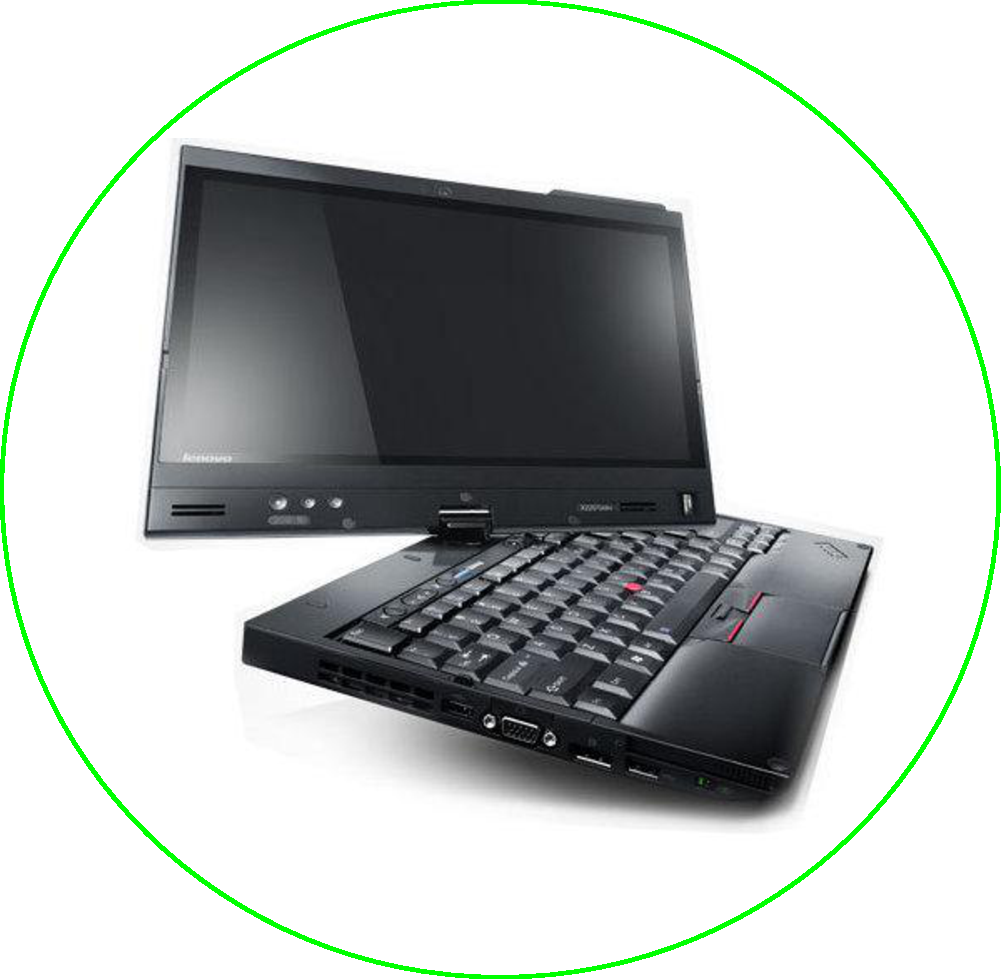
\includegraphics[width=0.25\textwidth]{x220t_hero_encircled}
			\begin{center}Tablet \end{center}}
			\hspace{0.05 \textwidth}
			\parbox[b]{0.28\textwidth}{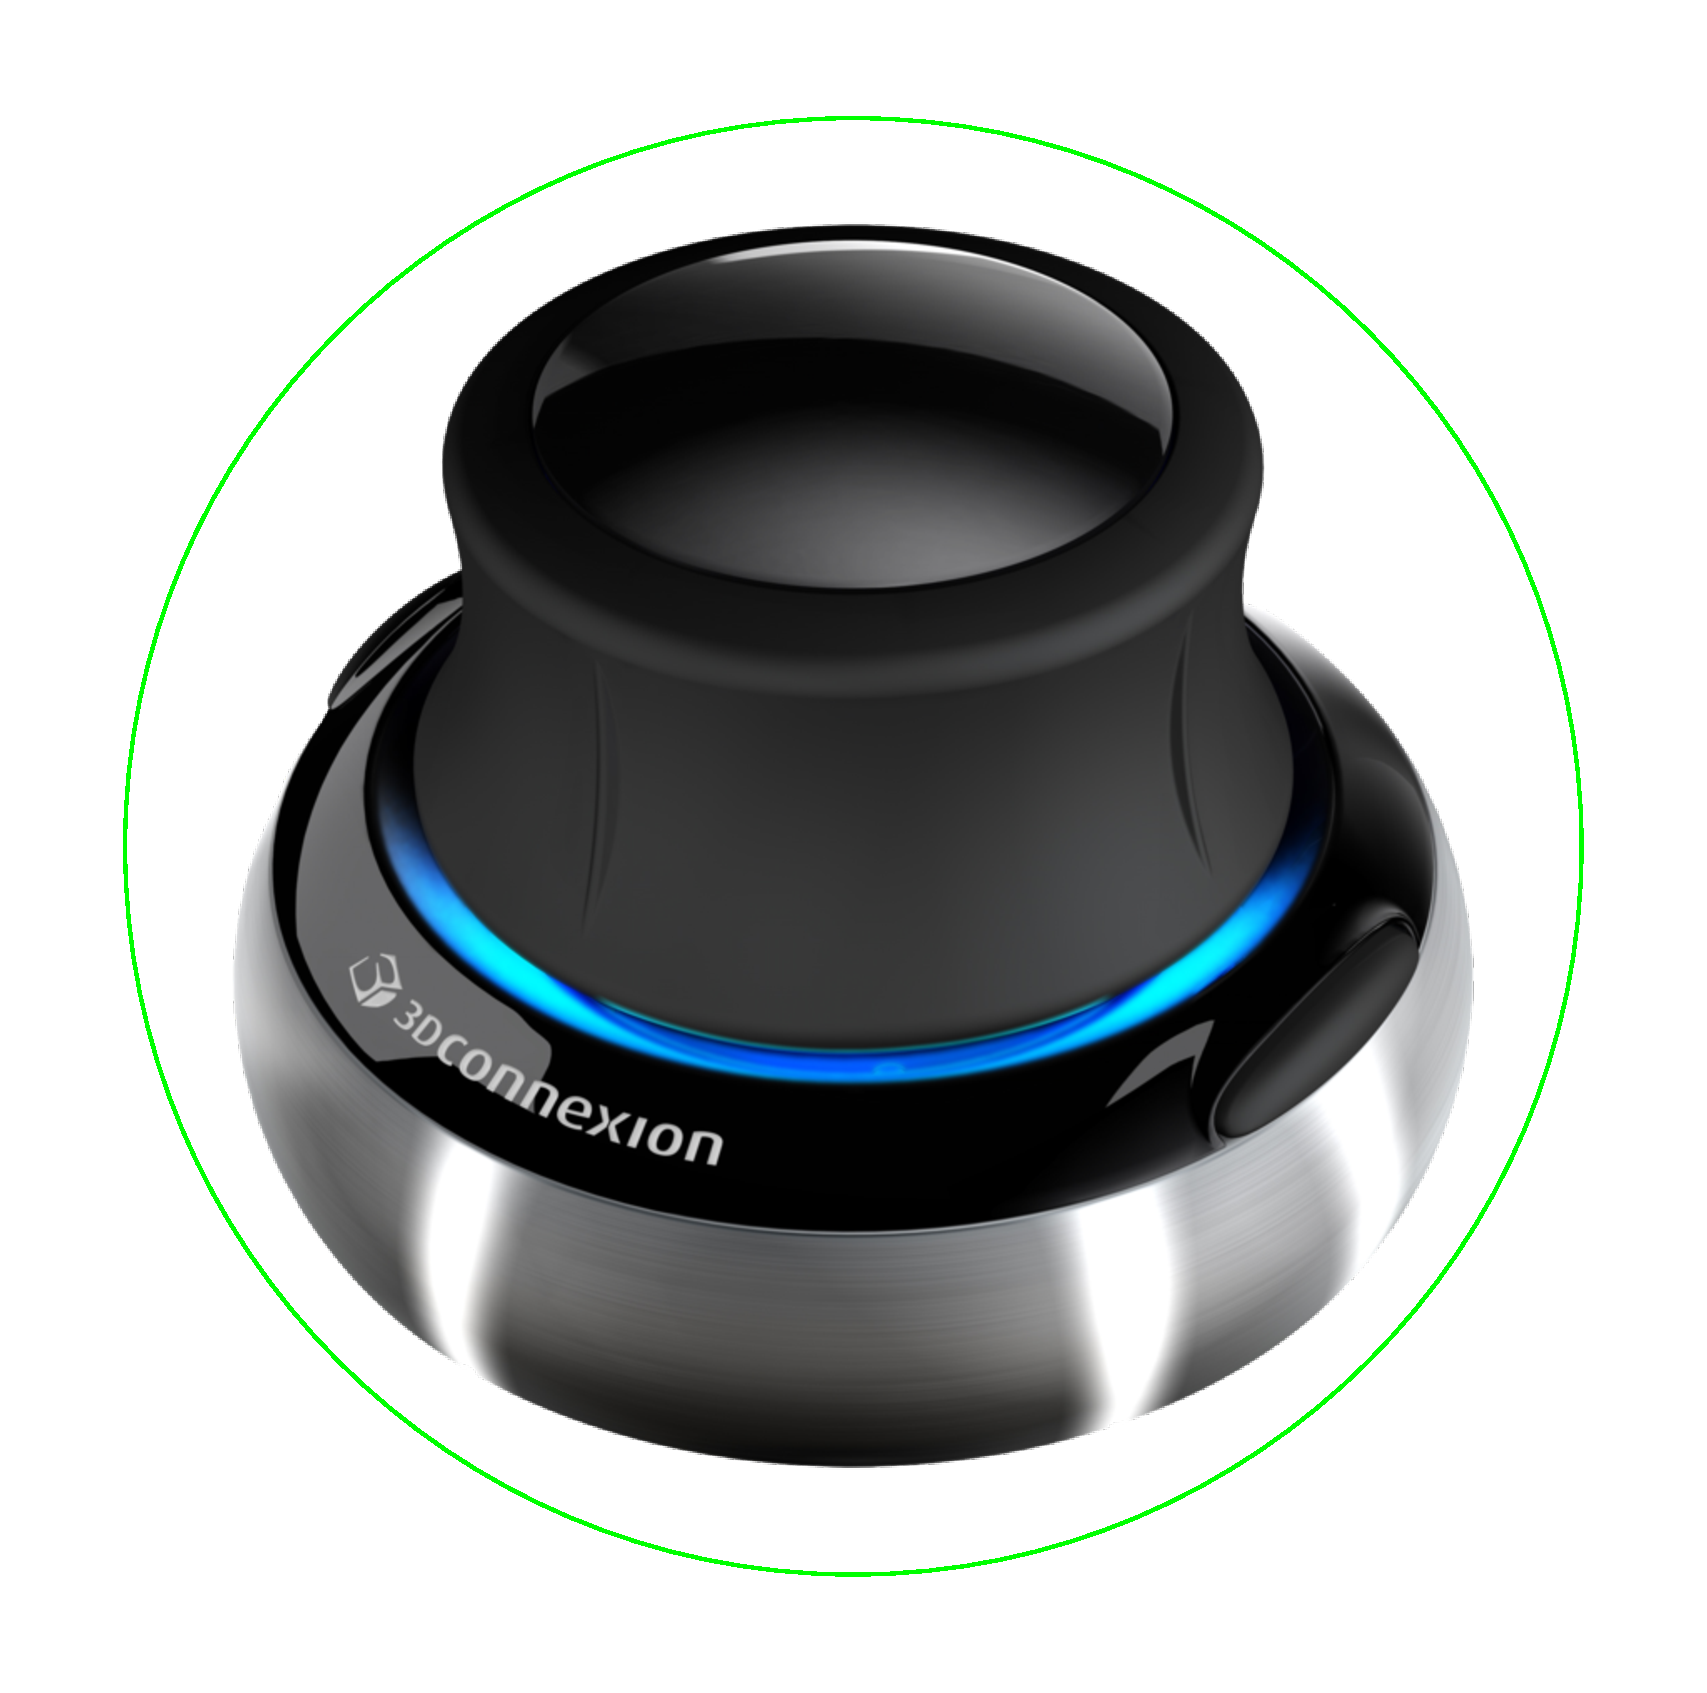
\includegraphics[width=0.28\textwidth]{3dx_productimage_encircled}
			\begin{center}3D mouse \end{center}}			
			\vspace{0.005\textwidth}
			\hspace{0.05\textwidth}			
			\parbox[b]{0.25\textwidth}{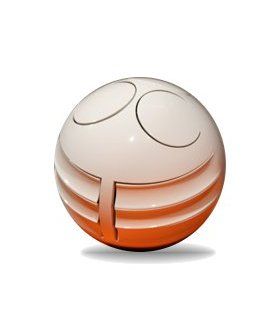
\includegraphics[width=0.25\textwidth]{qgo_sphere_cut}
			\begin{center}Qgo Sphere \end{center}}
			\hspace{0.05\textwidth}
			\parbox[b]{0.25\textwidth}{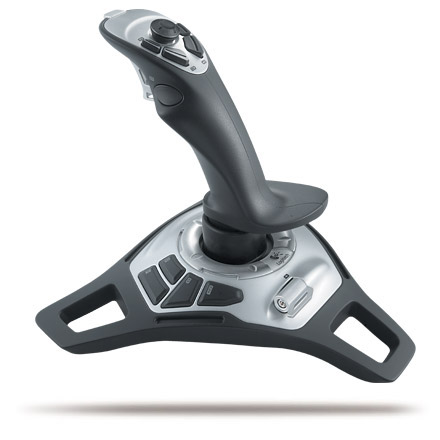
\includegraphics[width=0.25\textwidth]{Logitech-Freedom-Cordless-Joystick}
			\begin{center}Joystick \end{center}}
			\caption{The considered devices whereas the tablet with attached 3D mouse finally was chosen. The RC serves as a backup.}
			\label{fig:devices taken into consideration}	
		\end{center}
	}			
	\vspace{4.5mm}
\end{figure}

Table \ref{tab:requirements and expectations for hardware} shows the rating of the considered devices. It is visible that a solution in combination with a tablet had to be used, as only a tablet is able to fulfill the criteria for automatic controls and to run \textsc{ROS}. Although the Qgo Sphere\footnote{In  \cite{kammermann} the usage of the Qgo Sphere as an input device for a ballbot is discussed.} would be most intuitive to use with \textsc{Skye}, a 3D mouse (a space navigator from \textsc{3DConnection}) was chosen as a supplementary device to the tablet. Because of the fix-installed infrared sensors needed for the detection of the sphere's translational movements, the Qgo Sphere is not portable, which made it inconvenient to use for \textsc{Skye}. A joystick is not designed for six DOF and is therefore much less intuitive in use as a 3D mouse. For the tablet a \textsc{Lenovo} X220 was chosen as it can be transformed to a common notebook. This allows easy postprocessing of any gathered data. Additionally, a \textsc{Futaba} 7C RC serves as a backup in case of any breakdown within the main HMI.


\begin{table}[H]		% [H] indicates that the table should be right here.
	%\begin{tabularx}{\textwidth}{p{0.125\textwidth}p{0.2\textwidth}|p{0.06\textwidth}p{0.075\textwidth}p{0.08\textwidth}p{0.1\textwidth}p{0.08\textwidth}}	% add p{size_of_colomn} for every new column you'd like to have. If you put a | between the p then there is a vertical line between the columns. 
	\begin{center}
 \begin{tabular}{ll|ccccc}
\multicolumn{2}{l|}{Device}	& \rotatebox{90}{\mbox{RC}} 	& \rotatebox{90}{\mbox{Tablet}} 	&\rotatebox{90}{\mbox{3D Mouse}}	&\rotatebox{90}{\mbox{Qgo Sphere}}	&\rotatebox{90}{\mbox{Joystick}}  \\
	\toprule[1.25pt]				%define the line thickness of the top rule
	\multicolumn{2}{l|}{Stand alone}							&$\checkmark$		&$\checkmark$		&-			&-			&-\\
	\hline%\midrule
	\multirow{5}{*}{Matching}		&Test Phase					&-				&$\checkmark$		&-			&-			&-\\
									&Direct Control				&$\checkmark$		&$\checkmark$		&$\checkmark$	&$\checkmark$	&$\checkmark$ \\
									&Assisted Control			&$\checkmark$		&$\checkmark$		&$\checkmark$	&$\checkmark$	&$\checkmark$ \\
									&Half Automatic Control		&-				&$\checkmark$		&-			&-			&- \\
									&Full Automatic Control		&-				&$\checkmark$		&-			&-			&-\\
	
	\hline%\midrule
	\multicolumn{2}{l|}{Live View}							&-				&$\checkmark$		&-			&-			&-\\
	\hline%\midrule
	\multicolumn{2}{l|}{Intuitive}								&quite	&quite	&very&most&quite\\
	\hline%\midrule
	\multicolumn{2}{l|}{Portable}								&most	&quite	&quite&not &quite\\
		
	\bottomrule[1.25pt]
	%\end{tabularx} 
	\end{tabular}
	\caption[Requirements and Expectations for the Hardware]{Requirements and Expectations for the Hardware}
	\label{tab:requirements and expectations for hardware}
	\end{center}
\end{table}


\subsection{Software}
%\textit{QGroundControl, OpenPilot, Qt-Libraries} \\
\textsc{Google} and \textsc{Apple} showed how intuitive a GUI can be in combination with a  touchscreen with their operating systems for smartphones. They offer the user unknown flexibility in adopting the GUI to his needs. However, out of \textsc{Windows}, \textsc{Ubuntu}, \textsc{Mac OS}, \textsc{iOS} and \textsc{Android}, \textsc{Ubuntu} was the only operating system which provides complete support for \textsc{ROS}. Therefore \textsc{Ubuntu 11.10} was chosen as the operating system for the tablet.\\
As it was clear that there was no GUI ready to use unchanged for the HMI, open source software was analyzed in order to adopt it for \textsc{Skye}. Using \textsc{QGroundControl} (described in section \ref{subsec:qGroundControl}) was the best option. On the one hand it already offered the commonly used tools to control a UAV and on the other hand a good support in adopting it to the needs of \textsc{Skye} was granted as it was developed at the \textsc{ETH}.


\section{Realization}
\label{sec:realization}

\subsection{Compact and Convenient Solution}
Using a 3D mouse in combination with a tablet computer has a lot of advantages. Both devices can be put on a board with suspenders. Like this, the pilot has a compact portable control unit, without any external hardware interconnected (compare figure \ref{fig:HMI_in_Action}). While the 3D mouse provides intuitive control of the six DOF, the tablet with its GUI is used to filter and route the signals of the 3D mouse or serves as a highly modular touch input device on its own. With \textsc{QGroundControl} running on it, it also enables the pilot to adjust the controller and to set waypoints, while during the whole flight the live view of \textsc{Skye} is displayed (More on that in section \ref{subsec:qGroundControl}). In case the tablet should crash, the RC can be used to bring down \textsc{Skye} safely to ground.

\begin{figure}[H]
	\begin{center}
		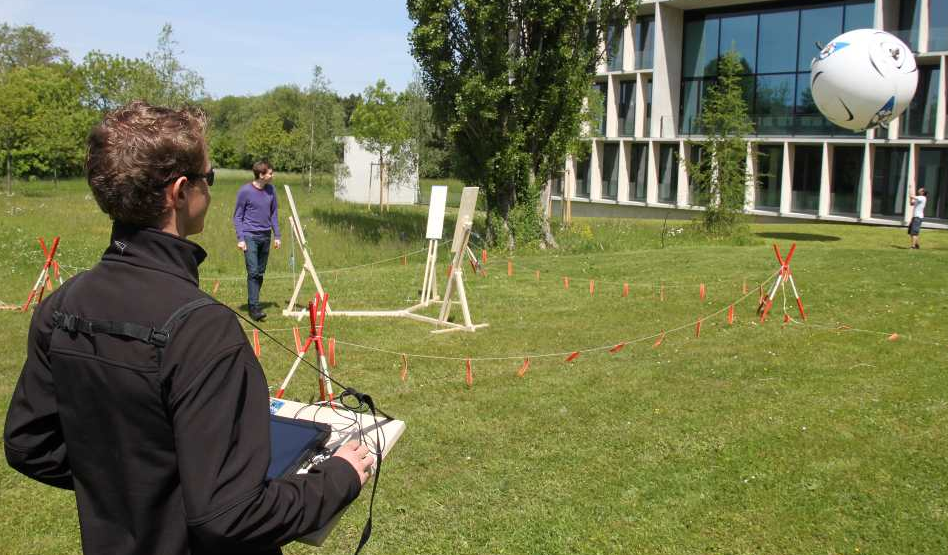
\includegraphics[width=0.85\textwidth]{graphics/HMI_in_Action}
		\caption{The compact, portable control unit in action}  
		\label{fig:HMI_in_Action}
	\end{center}
\end{figure}



\subsection{QGroundControl}
\label{subsec:qGroundControl}
%\textit{Adaptions in QGroundControl, 3dMouse, Touchscreen, Splines and Trajectory Controller \\ Only how it looks like and how to use. All ``important'' widgets are shown in detail. Implementation of 3dMouse and Touchscreen are not described further.picture of touch in action, mail final presentation}

The GUI \textsc{QGroundControl} for controlling unmanned vehicles was initially developed for \textsc{Pixhawk}\footnote{For more information on this project, see \url{https://pixhawk.ethz.ch/}.}, a vision based UAV project at the informatics department of \textsc{ETH}. It is a complete open source project based on Qt, which is a cross-platform-framework for GUIs written in \verb!C++!. For this thesis, the complete \textsc{QGroundControl} source code was taken and adopted for the needs of project \textsc{Skye}. This varied from adding single lines to develop complete new additional widgets\footnote{Widgets are kind of subwindows of the application.}. These widgets are described below. Inspiration and know-how was taken from \cite{blanchette} and nice tutorials and samples on \url{http://qt.nokia.com/}. In the following it is explained, how the control modes, defined in chapter \ref{cha:DifferentControlModes}, were realized with the chosen devices and with the GUI \textsc{QGroundControl}\footnote{The full automatic control mode was only simulated in \textsc{Matlab} and therefore no support of the GUI exists.}. 
\\
%\textbf{HERE matthias would like to summarize the basic code structure of qgc.. so it can be refered to and from the \textsc{Mavlink} section} 
%\\
To allow full control of system \textsc{skye}, a derived subclass to handle system specific procedures had to be programmed. 
This had to be done within compatibility to the messages defined in the \textsc{Mavlink} protocol (see section \ref{subsec:mavlink}). Precompiler commands have been used for cross-platform compatibility and \textsc{Skye} system specifications. 
With the Qt specific signals/slots interface the \textsc{Skye} subclass has been connected with the communication link as well as the user interfaces. 
An event handler has been integrated using the 3DxWare API, the official development kit for the used 3D mouse.

\subsubsection{The Main Control Widget}
With five different control modes (Test Phase, Direct Control (DC), Assisted Control (AC), Half Automatic Control (HAC), Full Automatic Control (FAC)) and three different input option (3D Mouse, Touchscreen, Keyboard), a main control widget was needed to choose between these options (see figure \ref{fig:qgc_skye_control} for its appearance). 
%With it the pilot can choose the control mode\footnote{As the Test Phase is not a usual control mode, its widget has to be opened in the menu bar.} and the input option.
The Test Phase mode is not meant to be used in flight and has therefore be activated via the menu bar.
The two sliders visible in figure \ref{fig:qgc_skye_control} allow to adjust the input scaling for translations and rotations respectively. Indoor flights need usually smaller but more accurate inputs, while outdoors more power is needed. The colored arm/disarm button is used to (de-)activate the actuators. At the same time it serves as an emergency button.

\begin{figure}[H] % [H] steht dafür, dass das Bild genau hier im Text sein soll.
	\begin{center}
		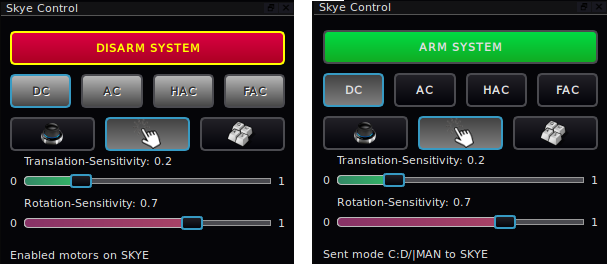
\includegraphics[width=0.7\textwidth]{qgc_skye_control}
		\caption{The main control widget in which most modes and options can be set. On the right its appearance with activated actuators and and the left its appearance with deactivated actuators.}
		\label{fig:qgc_skye_control}		
	\end{center}
\end{figure}



\subsubsection{Test Phase Control}
In order to test \textsc{Skye}'s four actuators before flight and in the development process, another widget was developed. It allows to adjust each of the eight actuation inputs separately. The input for the four thrusters is set by sliders and the orientation is set by turning the knobs. Again, there is a main button (Activate Engine) to start and stop the motors.

\begin{figure}[H] % [H] steht dafür, dass das Bild genau hier im Text sein soll.
	\begin{center}
		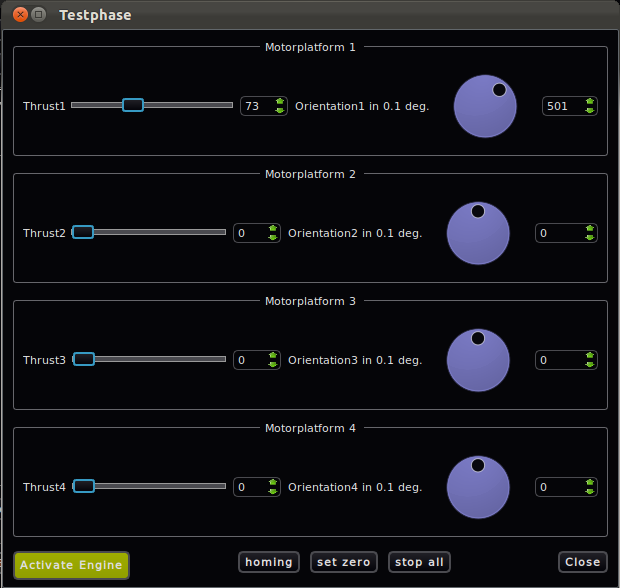
\includegraphics[width=0.7\textwidth]{qgc_test_phase}
		\caption{The test phase widget }  
		\label{figure:qgc_test_phase}
	\end{center}
\end{figure}


\subsubsection{Direct Control}
The main device for the direct control mode is the 3D mouse which is connected by USB to the tablet. To use its input signals in  \textsc{QGroundControl}, a interface had to be written. With the two knobs on the device (hardly visible in figure \ref{fig:3D_mouse}) the pilot is able to (de-)activate translational or rotational inputs. This allows a very precise control.

\begin{figure}[H] % [H] steht dafür, dass das Bild genau hier im Text sein soll.
	\begin{center}
		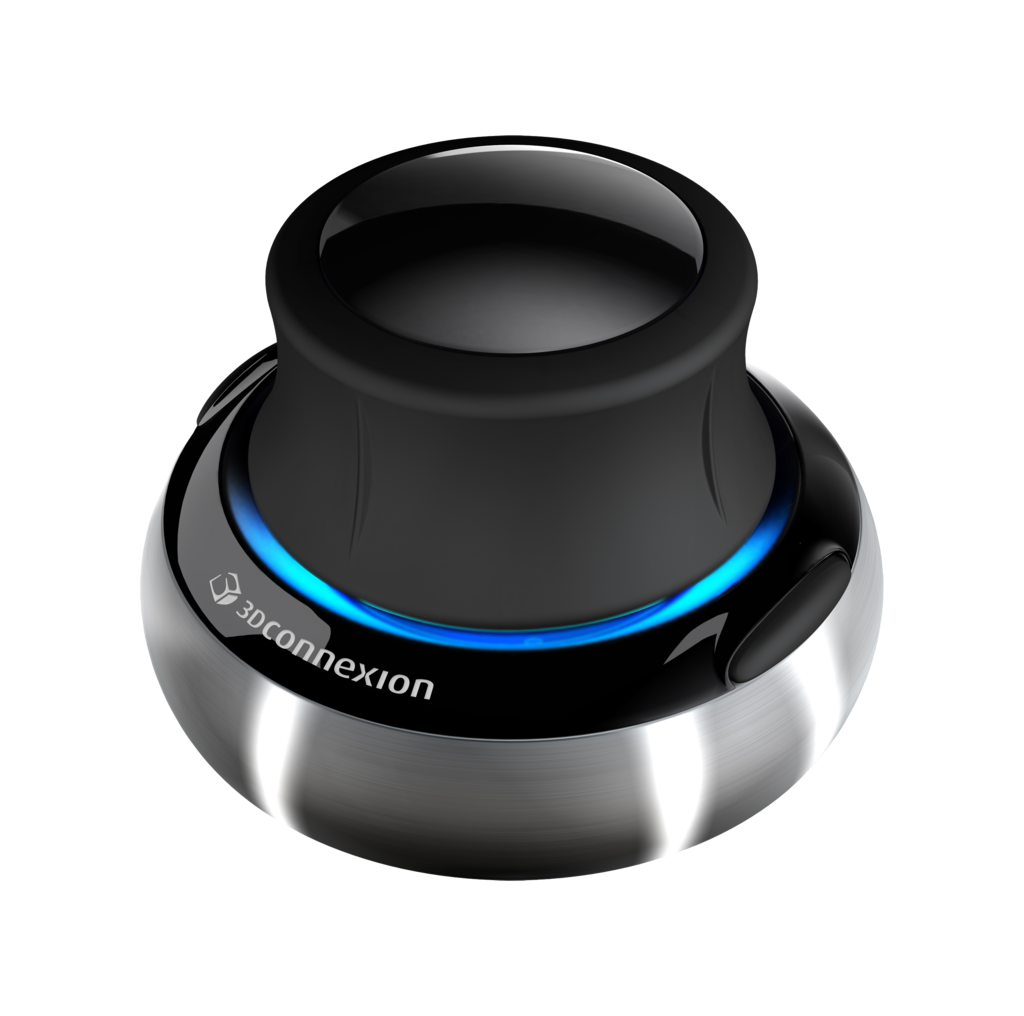
\includegraphics[width=0.4\textwidth]{3dx_productimage}
		\caption{The 3D mouse used for the direct control }  
		\label{fig:3D_mouse}
	\end{center}
\end{figure}

\subsubsection{Assisted Control}
\label{subsub:assistedcontrol}
Feeding velocities instead of a force and a moment makes the usage of the touchscreen beside the 3D mouse more reasonable. For this mode a combination of different widgets is used, shown in figure\footnote{This screenshot is a reproduced situation of the flight in ETH main building. Obviously, no GPS information were available then.} \ref{fig:qgc_manual_control}. The widgets can be scaled and positioned individually. As a default view for \textsc{Skye}, the shown arrangement of the Head-up-Display (HUD), map and main control widget is provided. If touch input is chosen, the HUD enables rotational touch inputs directly on the displayed live view. The map widget shows the position of \textsc{Skye} and allows to set translational inputs. Note that in a first approach these inputs were always interpreted in the camera frame as the state estimation was not yet running. Intuitively, this has to be transformed to inputs in the North-East-Down (NED) frame which has recently been tested on the system.

\begin{figure}[H] % [H] steht dafür, dass das Bild genau hier im Text sein soll.
	\begin{center}
		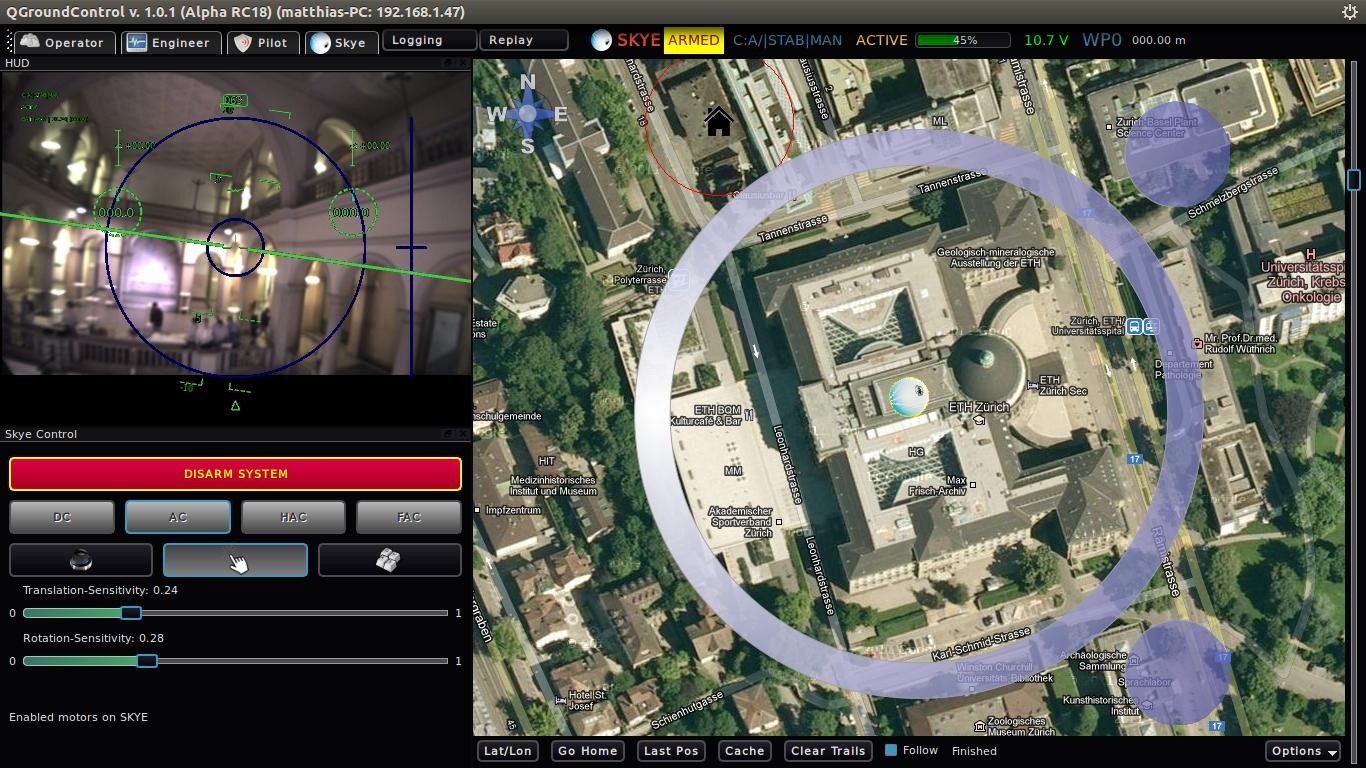
\includegraphics[width=0.8\textwidth]{qgc_manual_control}
		\caption{The pilot's view on the GUI if assisted  control and touch input is activated.}  
		\label{fig:qgc_manual_control}		
	\end{center}
\end{figure}

\begin{figure}[H] % [H] steht dafür, dass das Bild genau hier im Text sein soll.
	\begin{center}
		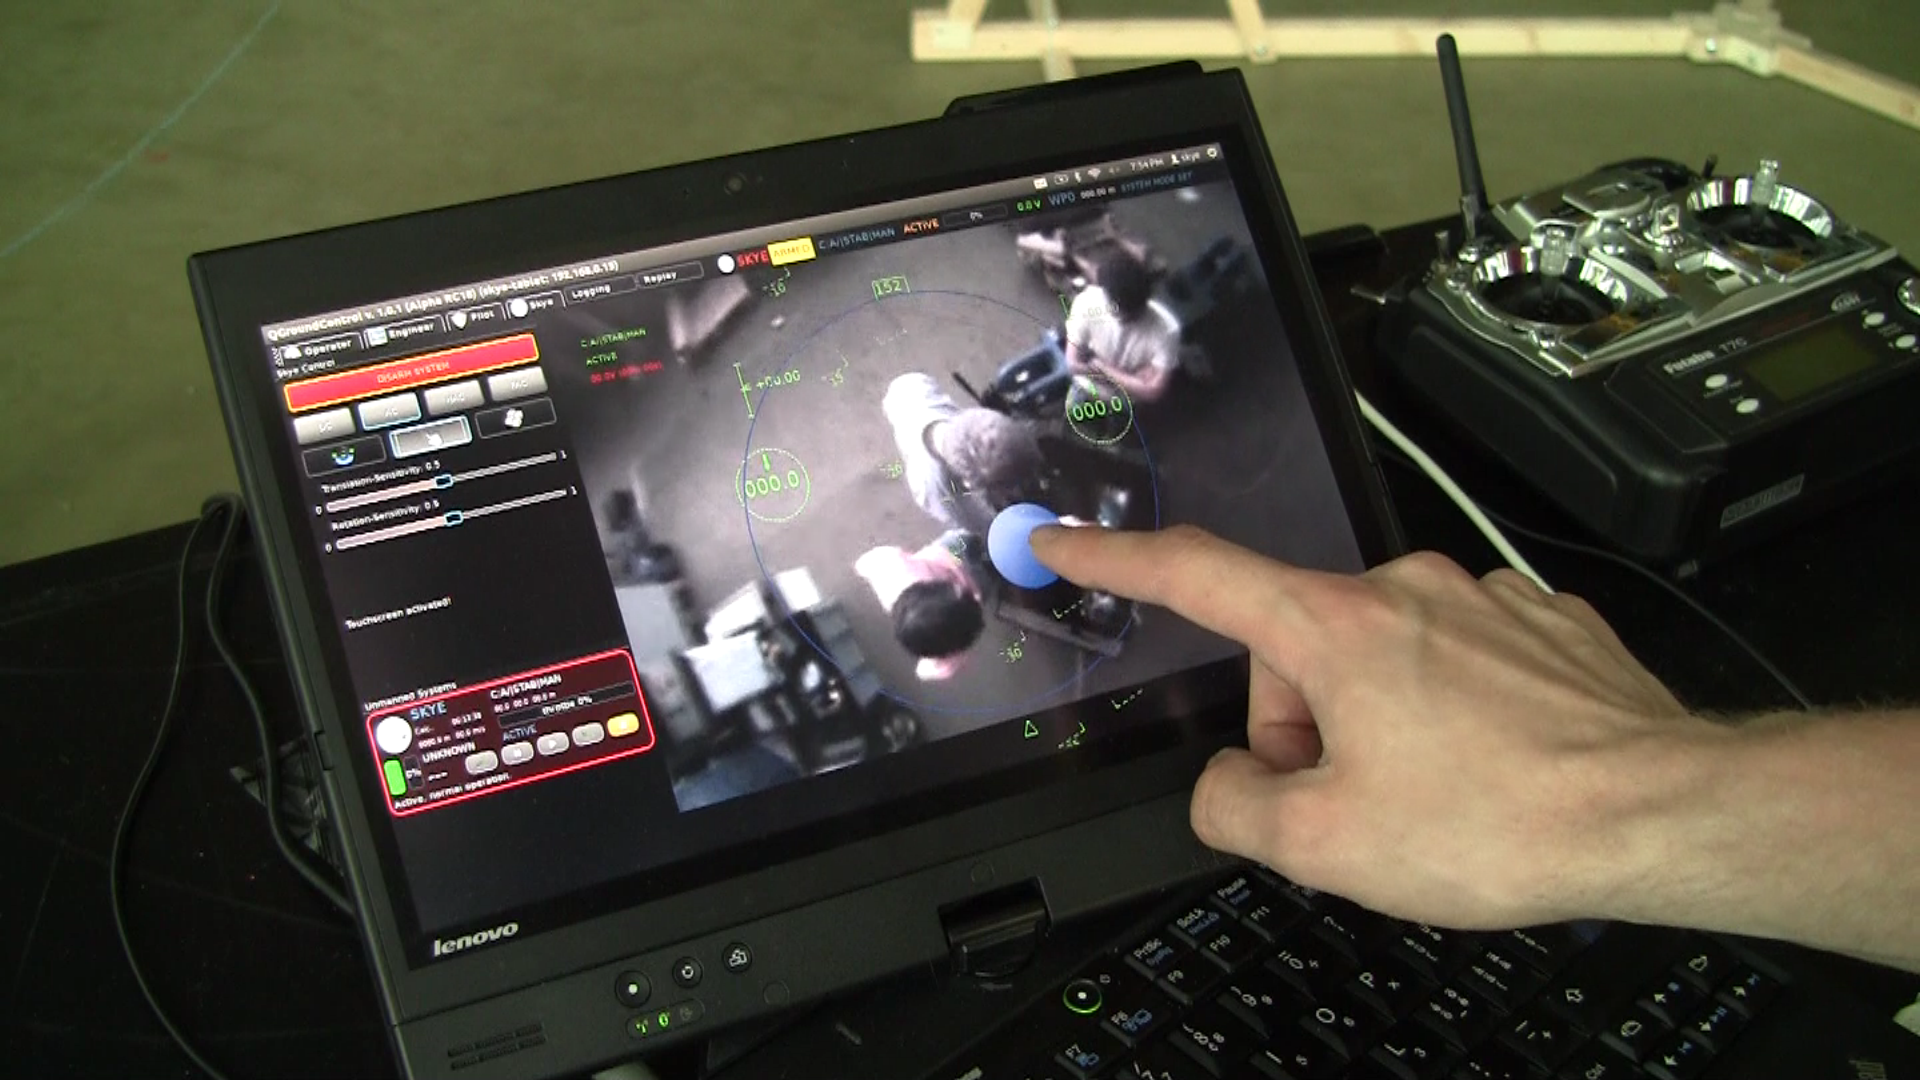
\includegraphics[width=0.8\textwidth]{graphics/TouchInput}
		\caption{The enlarged HUD with touch input in action}  
		\label{fig:touchInput}		
	\end{center}
\end{figure}


\subsubsection{Half Automatic Control}
\label{subsub:halfautomaticcontrol}
For this mode a trajectory is needed. Therefore \textsc{QGroundControl} was adopted to generate it. After setting the waypoints on Google Maps, the user can adjust the their height over ground. In order to properly display the elevation, the Google Elevation API\footnote{\url{https://developers.google.com/maps/documentation/elevation/}}was used. Once the waypoints are set an interpolating cubic spline is calculated and displayed (see figure \ref{fig:qgc_automatic_control}). Out from the recent position of \textsc{Skye}, a velocity input is calculated using a \textit{Pure Pursuit} approach\footnote{In section \ref{sub:pure_pursuit} \textit{Pure Pursuit} is described how it was implemented in \textsc{Matlab}.} The part of the path that is already reached is displayed in blue. The methods for waypoint interpolation and trajectory generation are describe in more detail in chapter \ref{cha:trajectory}.% The trace of the (simulated) motion is tracked with red dots.

\begin{figure}[H] % [H] steht dafür, dass das Bild genau hier im Text sein soll.
	\begin{center}
		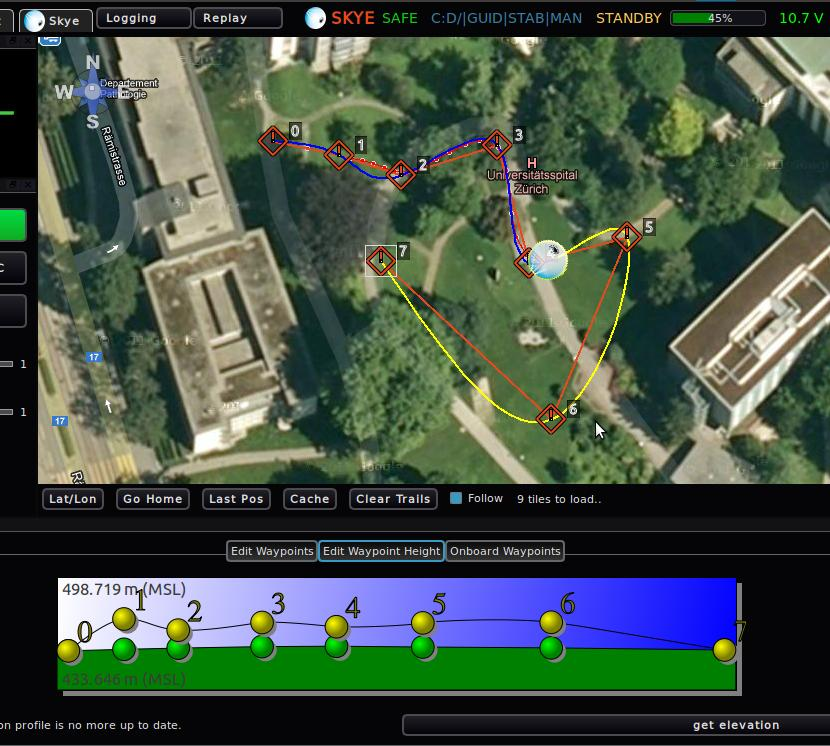
\includegraphics[width=0.8\textwidth]{qgc_automatic_control}
		\caption{Generating a trajectory with the GUI}
		\label{fig:qgc_automatic_control}		
	\end{center}
\end{figure}

%\textbf{A Picture of the DC/AC widget should be placed at least in the APENDIX.. Camera reconfiguration and battery info can be left away.}

Further on, widgets to adjust camera properties, displaying detailed battery info or to set Direct or Assisted Control to exact values via sliders have been added. Despite of the latter\footnote{The Direct/Assisted Control widget has been used to enable the system verifications in \cite{meiermueri} and \cite{weichart}.} they could not be used in practice. The Direct/Assisted Control widget is shown in figure \ref{fig:qgc_manual_control_widget}.

\subsection{Mavlink}
\label{subsec:mavlink}
%\textit{Summary of Protocal, adaptions and use for} \textsc{Skye} \\
Mavlink (Micro Air Vehicle Communication Protocol) is a very lightway header-only message marshalling library for micro air vehicles\footnote{Official description from \url{http://qgroundcontrol.org/mavlink/start}}. It is a widely used protocol geared for transmission speed and safety. A mavlink packet consists of a six byte prefix including start byte, payload length and sequence number as well as component, system and message ID. A two byte suffix checksum is used. The payload size is maximum 255 bytes. Many autopilots as well as cross-platform software packages are using Mavlink.
A set of commonly used messages is provided. The protocol had to be extended for the convenient use with \textsc{Skye} (an example\footnote{The full xml file including the message definitions for \textsc{Skye} is in the appendix (listing \ref{app_xml}).} of such a message definition is shown in listing \ref{xml_assisted_control}). This can be done by defining the additional messages in a xml script. The C-headers will be generated by the Mavlink Generator. The control commands, system telemetry as well as image live stream for \textsc{Skye} are transmitted using Mavlink protocol. For the transmission of waypoints, an extended waypoint protocol is provided by Mavlink. The waypoints set on the map widget and height profile (see section \ref{subsub:halfautomaticcontrol}) as well as the autopilot (\textit{PX4FMU}) are compatible to this protocol.

\begin{lstlisting}[captionpos=b, caption=Sequence of skye.xml: Definition of the Assisted Control command Mavlink message. It consists of six 32 bit floating numbers for the input values and a 8 bit integer to indicate the target system's ID (the GUI could actually be connected to more than one UAV at the same time)., label=xml_assisted_control]
<message id="155" name="SKYE_ASSISTED_CONTROL">
   <description>Control six degrees of freedom. Translational velocity in Inertial (earth) Frame. Use this manual control mode with the requested mode: 
"MAV_MODE_ASSISTED_CONTROL_ARMED"</description>
   <field type="uint8_t" name="target_system">System ID</field>
   <field type="float" name="translation_lat">Translation (velocity) in Inertial Frame latitude, in m/sec</field>
   <field type="float" name="translation_long">Translation (velocity) in Inertial Frame longitude, in m/sec</field>
   <field type="float" name="translation_alt">Translation (velocity) in Inertial Frame altitude, in m/sec</field>
   <field type="float" name="rotation_x">Roll (angular velocity), in rad/sec</field>
   <field type="float" name="rotation_y">Pitch (angular velocity), in rad/sec</field>
   <field type="float" name="rotation_z">Yaw (angular velocity), in rad/sec</field>
</message>
\end{lstlisting}
